% Copyright 2021 Edoardo Riggio

% Licensed under the Apache License, Version 2.0 (the "License");
% you may not use this file except in compliance with the License.
% You may obtain a copy of the License at

% 	http://www.apache.org/licenses/LICENSE-2.0

% Unless required by applicable law or agreed to in writing, software
% distributed under the License is distributed on an "AS IS" BASIS,
% WITHOUT WARRANTIES OR CONDITIONS OF ANY KIND, either express or implied.
% See the License for the specific language governing permissions and
% limitations under the License.

\documentclass{article}

\usepackage{hyperref, amsmath, graphicx, amssymb, csquotes, tabularx}
\usepackage{fancyvrb,newverbs,xcolor}

\graphicspath{ {./assets/} }

\definecolor{cverbbg}{gray}{0.93}

\newenvironment{cverbatim}
 {\SaveVerbatim{cverb}}
 {\endSaveVerbatim
  \flushleft\fboxrule=0pt\fboxsep=.5em
  \colorbox{cverbbg}{\BUseVerbatim{cverb}}%
  \endflushleft
}

\newenvironment{lcverbatim}
 {\SaveVerbatim{cverb}}
 {\endSaveVerbatim
  \flushleft\fboxrule=0pt\fboxsep=.5em
  \colorbox{cverbbg}{%
    \makebox[\dimexpr\linewidth-2\fboxsep][l]{\BUseVerbatim{cverb}}%
  }
  \endflushleft
}

\newcommand{\ctexttt}[1]{\colorbox{cverbbg}{\texttt{#1}}}
\newverbcommand{\cverb}
  {\setbox\verbbox\hbox\bgroup}
  {\egroup\colorbox{cverbbg}{\box\verbbox}}

\begin{document}
\begin{titlepage}
    \begin{center}
        \vspace*{1cm}
        
        \Huge
        \textbf{Artificial Intelligence Cheatsheet}
        
        \vspace{0.5cm}
        \LARGE
        
        \vspace{.5cm}
        
        Edoardo Riggio
   		  \vspace{1.5cm}
       
        \vfill
        
        \today
        
        \vspace{.8cm}
          \Large
          Artificial Intelligence - S.A. 2021 \\
        Computer Science\\
        Universit\`{a} della Svizzera Italiana, Lugano\\
        
    \end{center}
\end{titlepage}

\tableofcontents

\newpage

\section{Blind Search Algorithms}
A \textbf{search algorithm} takes as input a problem space and a starting state, and tries to compute a path in the best possible way. \\ \\
The strategy is to search which node to expand among the yet undiscovered nodes. In order to expand a node, we need to consider all of the nodes that are reachable in one step from the selected node.

\subsection{Definitions}
\subsubsection{Search Tree}
A search tree is a tree composed of nodes. Each node in the tree represents a step in the search algorithm. A node is composed of:

\begin{itemize}
	\item State
	\item Node who generated it
	\item Action used to generate it
	\item Depth of the tree
	\item Cost of the path from the root
\end{itemize}

\subsubsection{Travelling Salesman Problem}
The goal of this problem is to visit all the cities of a graph such that the travelling cost is minimum. The travelling cost is measured by summing up all of the travelling costs from the starting city to the destination city.

\subsubsection{Evaluation of Search Strategies}
There are four common criteria for evaluating search strategies:

\begin{itemize}
	\item \textbf{Completeness}
	\vspace{.2cm} \\
	Does the algorithm always find a solution if one exists?
	
	\item \textbf{Optimality}
	\vspace{.2cm} \\
	Does the algorithm guarantee the least-cost solution?
	
	\item \textbf{Time Complexity}
	\vspace{.2cm} \\
	How much time does it take for an algorithm to run?
	
	\item \textbf{Space Complexity}
	\vspace{.2cm} \\
	How much memory does the algorithm require?
\end{itemize}

\subsection{Breath-First Search}
In this algorithm, the shallowest unexpanded node is expanded. In order to do so, this algorithm requires a FIFO queue. This type of queue is able to keep track of which node to expand next. \\

\begin{center}
	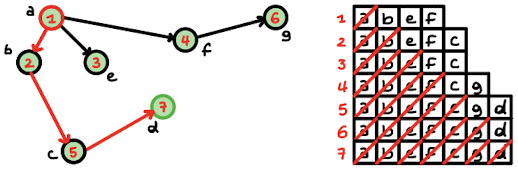
\includegraphics[width=9cm]{bfs.png}
\end{center}
\vspace{.3cm}
This algorithm is \textbf{complete}. It is also \textbf{optimal} in the case that all of the steps have the same cost. Furthermore, the \textbf{space and time complexities} of this algorithm are both $O(b^d)$. Where $b$ is the branching factor, and $d$ is the solution depth.

\subsection{Uniform-Cost Search}
In this algorithm, a cost is assigned to each edge of the graph. Here a node is expanded if $g(n)$ -- i.e. the distance from the root to the node -- is minimal. \\

\begin{center}
	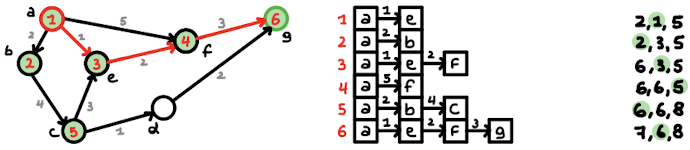
\includegraphics[width=12cm]{ucs.png}
\end{center}
\vspace{.3cm}
In the above image, on the far right we have the values of $g(n)$ at each step, while in the middle, we have the path chosen at each step. \\ \\
This algorithm is \textbf{complete}. It is also \textbf{optimal} in the case that all costs are non-negative. Furthermore, the \textbf{space and time complexities} are both $O(b^d)$, where $b$ is the branching factor, and $d$ is the solution depth.

\subsection{Depth-First Search}
This algorithm expands the deepest unexpanded node. In order to do so, it uses a LIFO queue. \\

\begin{center}
	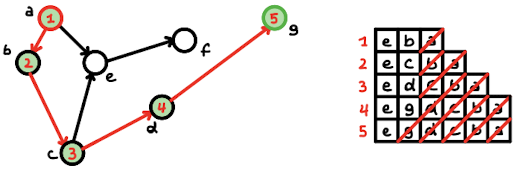
\includegraphics[width=9cm]{dfs.png}
\end{center}
\vspace{.3cm}
This algorithm is \textbf{not complete} in the case of an infinite state space -- since it has no depth limitation. It is also \textbf{not optimal}. Furthermore, the \textbf{time complexity} of the algorithm is $O(b^m)$, while the \textbf{space complexity} is $O(b \cdot m)$. Where $b$ is the branching factor and $m$ is the maximum depth of the search tree.

\subsection{Depth-Limited Search}
In this case we have an algorithm which is identical to the DFS search. The only difference between the two is that depth-limited search is -- as the name suggests -- limited. This means that it will stop when it reaches a certain depth in the solution tree. \\ \\
This algorithm is \textbf{complete} in the case where we know a bound to the solution depth. It is \textbf{not optimal}. Furthermore, the \textbf{time complexity} is $O(b^d)$, and the \textbf{space complexity} is $O(b \cdot d)$. Where $b$ is the branching factor and $d$ is the maximum depth.

\subsection{Iterative Deepening Search}
This is a depth-limited search algorithm, where at each step, a counter representing the tree's depth is incremented. DFS is performed at every repetition of the algorithm -- when the algorithm goes back to the starting node, and it stops at the depth indicated by the counter. \\ \\
This algorithm is \textbf{complete}. It is also \textbf{optimal} in the case that there are non-negative costs. Furthermore, the \textbf{time complexity} is $O(b^d)$, and the \textbf{space complexity} is $O(b \cdot d)$. Where $b$ is the branching factor and $d$ is the depth at which the goal is found.

\subsection{Bi-Directional Search}
This algorithm considers two queues, one only containing the root, and one only containing the goal. The nodes of each queue are expanded until both queues contain a common node. \\ \\
This algorithm is both \textbf{complete} and \textbf{optimal}. Furthermore, the \textbf{time and space complexities} are $O(b ^{\frac{d}{2}})$, where $b$ is the branching factor, and $d$ is the depth at which the goal is located.

\section{Heuristic Search Algorithms}
\textbf{Heuristic knowledge} helps to execute good choices. It does not avoid search, but it reduces it. It is used when a problem has exponential complexity -- i.e. is NP-complete. \\ \\
This knowledge is given by a state evaluation function, called the \textbf{heuristic evaluation}.

\subsection{Definitions}
\subsubsection{Admissible Heuristic}
A heuristic is said to be admissible if it never overestimates the cost of reaching the goal -- i.e. the cost estimated to reach the goal is not higher than the lowest possible cost from the current node.

\[ \forall n~|~h(n) \leq h^*(n) \] \\
Where $n$ is a node, $h$ is a heuristic, $h(n)$ is the cost from node $n$ to the goal -- defined by $h$, and $h^*(n)$ is the optimal cost from $n$ to the goal.

\subsubsection{Monotonic Heuristic}
A heuristic is said to be monotone if, for each node $n$ and its successor $n'$, the estimated cost of reaching the goal from $n$ is no longer greater than the step cost of getting to $n'$ plus the estimated cost of reaching the goal from $n'$.

\[ f(n) \leq f(n') \] \\
Where $f(n)$ is the cost from the root to node $n$ plus the cost estimation from node $n$ to the goal. Same thing goes for $f(n')$. A monotonic heuristic is always admissible. Not all admissible heuristics are monotonic. In addition, all monotonic heuristics guarantee local optimality.

\subsection{Best-First Search}
Each node of the graph is evaluated by estimating its distance to the goal. The node which has the shortest distance to the goal is selected to be expanded.\\

\begin{center}
	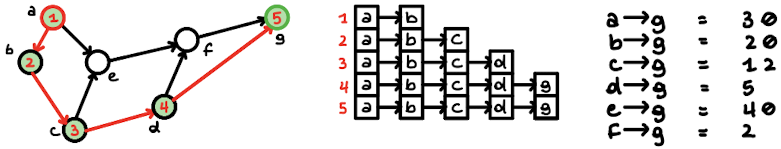
\includegraphics[width=12cm]{befs.png}
\end{center}
\vspace{.3cm}
Where on the far right we have all the values given by the heuristic function $h$. \\ \\
This algorithm is \textbf{not complete} and \textbf{not optimal}. Furthermore, the \textbf{time complexity} and \textbf{space complexity} are both $O(b^m)$. Where $b$ is the branching factor and $m$ is the depth of the search tree.

\subsection{A*}
The evaluation function for this algorithm is:

\[ f^*(n) = g^*(n) + h^*(n) \] \\
Where $f^*(n)$ is the estimated cost of the path from the root to the goal, $g^*(n)$ is the cost of the path from the root to node $n$, and $h^*(n)$ is the estimated cost of the path from node $n$ to the goal -- given by the heuristic $h$.\\

\begin{center}
	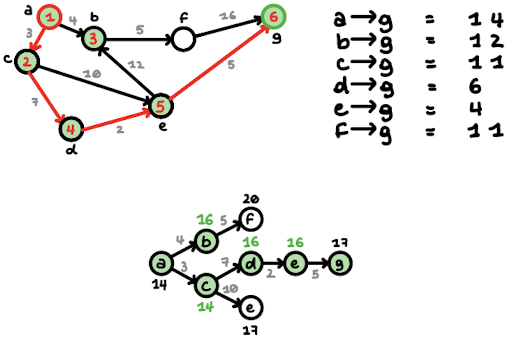
\includegraphics[width=9cm]{a*.png}
\end{center}
\vspace{.3cm}
This algorithm is \textbf{complete} -- unless there are infinitely many nodes with $f \leq f(G)$, where $G$ is the goal. It is also \textbf{optimal}. Furthermore, the \textbf{time complexity} and \textbf{space complexity} are both $O(b^m)$. Where $b$ is the branching factor and $m$ is the depth of the search tree.

\subsubsection{Optimality of A*}
Given that: \blockquote{If $A^*$ selects a path $p$, then $p$ is the shortest path -- i.e. least-cost path -- in order to reach the goal}, the optimality of $A^*$ can be demonstrated in the following way:

\begin{enumerate}
	\item Assume -- for contradiction -- that some other path $p'$ is actually the shortest path to a goal
	\item Consider that, before $p$ is chosen from the fringe, some part of path $p'$ will also be on the fringe. This partial path will be called $p''$
	\item Because $p$ was expanded before $p''$ was, then we will have:
	\[ f(p) \leq f(p'') \]
	\item Because $p$ is a goal, this means that $h(p) = 0$. Thus:
	\[ g(p) \leq g(p'') + h(p'') \]
	\item Because $h$ is admissible, this means that the following is true for any path $p'$ to a goal that extends $p''$:
	\[ g(p'') + h(p'') \leq g(p') \]
	\item We will thus obtain the following for any other path $p'$ to a goal:
	\[ g(p) \leq g(p') \]
	Which contradicts the assumption of $p'$ being the shortest path
\end{enumerate}

\subsection{IDA*}
This algorithm combines $A^*$ with iterative deepening. At each iteration of the algorithm, we perform DFS, pruning the branches in which its total estimated cost

\[ f(n) = g(n) + h(n) \] \\
Exceeds a given threshold. The value of this threshold starts as the value of $f$ of the initial node, and increases for each iteration of the algorithm. The next value of the threshold is computed as the minimum value of $f$ of all values that exceeded the current threshold. \\ \\
As for $A^*$, this algorithm is also both \textbf{complete} and \textbf{optimal}. Furthermore, the \textbf{time complexity} is $O(b^m)$, while the \textbf{space complexity} is $O(b \cdot m)$. Where $b$ is the branching factor and $m$ is the depth of the search tree.

\section{Constructive Greedy Search Algorithms}
A constructive greedy algorithm is based on the following steps:

\begin{enumerate}
	\item Start from a random node
	\item Expand the node in order to generate all possible next nodes
	\item Choose the next best node based on a local strategy
	\item Current solution is extended with the one found at point 3
	\item Repeat steps 2 through 4, until a feasible solution is computed
\end{enumerate}
These algorithms start from a feasible solution in a subset of the search space, and iteratively add elements to the partial solution -- according to some strategy -- until no node is left.

\subsection{Nearest Neighbour}
This is one of the most common algorithms used to solve TSP problems. The algorithm is the following:

\begin{enumerate}
	\item Consider a starting tour made up of a random node
	\item Add the city which is the closest to the previous city to the tour. The next city must not have been visited yet
	\item Repeat step 2 until no node is available
\end{enumerate}
The following is a graphical representation of the algorithm.\\

\begin{center}
	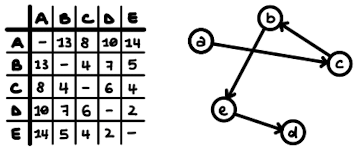
\includegraphics[width=6cm]{nn.png}
\end{center}
\vspace{.3cm}
Where on the right we have the connectivity matrix of the graph. Each non-zero element in the matrix represents the distance between two nodes $n_i$ and $n_j$. \\ \\
The \textbf{time complexity} of this algorithm is $O(n^2)$.

\subsection{Multi-Fragment}
This algorithm builds a tour as follows:

\begin{enumerate}
	\item Sort the edge costs in ascending order
	\item Select the first edge. This will be the first edge of the new tour
	\item Add new edge in incremental order only if it does not create a three-degree city -- i.e. does not create a cycle
	\item Repeat step 3 until no edge is available
\end{enumerate}
The \textbf{time complexity} of this algorithm is $O(n^2 \cdot \log n)$.

\subsection{Nearest Insertion}
This algorithm does the following:

\begin{enumerate}
	\item Build an initial tour formed by the nearest cities
	\item Choose a node that is not in the computed tour, such that the Euclidean distance between it and two other nodes in the tour is minimum
	\item Insert the new node between the two nodes of the tour
	\item Repeat steps 2 and 3 until there are no nodes left
\end{enumerate}
The \textbf{time complexity} of this algorithm is $O(n^2)$.

\subsection{Farthest Insertion}
This algorithm does the following:

\begin{enumerate}
	\item Build an initial tour formed by the farthest cities
	\item Choose a node that is not in the computed tour, such that the Euclidean distance between it and two other nodes in the tour is maximum
	\item Insert the new node between the two nodes of the tour
	\item Repeat steps 2 and 3 until there are no nodes left
\end{enumerate}
The \textbf{time complexity} of this algorithm is $O(n^2)$.

\section{Local Search Algorithms}
In the case of local search, we start from complete solutions. These solutions are then optimized by means of algorithms. The following is the general structure of this type of algorithms:

\begin{enumerate}
	\item Start from a complete solution
	\item Compute the first best edge exchange that improves the tour
	\item Execute the change
	\item Search for another change until no further improvement is possible
\end{enumerate}

\subsection{Hill Climbing}
This algorithm explores the entire neighbourhood, and searches for a better solution until no further improvement is possible. \\ \\
For each current solution, the algorithm evaluates all of its neighbours. If

\[ f(\text{next}) < f(\text{current}) \] \\
Where $f$ is an objective function. Then, the current solution will be substituted by the next solution.

\subsection{2-Opt}
This algorithm is used in order to remove crossings in the solution path. This is done by selecting two nodes which contains crossings between them, and reversing the path between these two nodes. \\

\begin{center}
	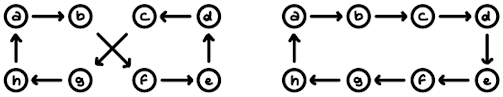
\includegraphics[width=9cm]{2opt.png}
\end{center}
\vspace{.3cm}
The \textbf{time complexity} of this algorithm is $O(n^2)$.

\subsection{2.5-Opt}
In this case, in addition to check is there are possible 2-opt swaps, we also check for two possible node shifts -- for node $n_i$ and $n_j$. A node swift is done by moving a node to another position in the tour. \\

\begin{center}
	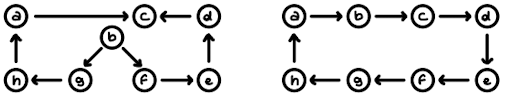
\includegraphics[width=9cm]{2.5opt.png}
\end{center}
\vspace{.3cm}
The \textbf{time complexity} of this algorithm is $O(n^2)$.

\subsection{3-Opt}
In this case, we remove three links form the tour, thus obtaining three segments to manipulate. With these three segments we check for possible multiple 2-opt swaps, as well as node shifts. \\

\begin{center}
	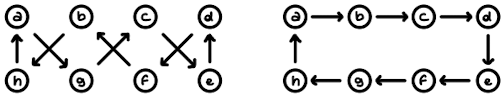
\includegraphics[width=9cm]{3opt.png}
\end{center}
\vspace{.3cm}
The \textbf{time complexity} of this algorithm is $O(n^3)$.

\section{Meta-Heuristic Search Algorithms}
The main problems with local search strategies are that a local minimum cannot be escaped, and they are inefficient when the neighbourhood is too large. \\ \\
A way to solve these problems is to do the following:

\begin{itemize}
	\item Stochastically explore only a subset of the neighbourhood
	\item Accept those solutions that are worst than the previous
\end{itemize}
Meta-heuristic algorithms are usually inspired by natural systems. Such algorithms are, for example:

\begin{itemize}
	\item Simulated annealing
	\item Genetic algorithms
	\item Ant colony optimization
\end{itemize}

\subsection{Simulated Annealing}
This algorithm is inspired by the natural annealing of metals. the algorithm follows these steps:

\begin{enumerate}
	\item Start from an initial current solution
	\item At each iteration, a new solution next is randomly chosen from the neighbourhood of the current solution
	\item If $f(\text{next}) < f(\text{current})$, then $f(\text{next})$ becomes the current node. Otherwise, we use a probabilistic function
	\[ e^{-\frac{\Delta E}{T}} \]
	Where $\Delta E = f(\text{next}) - f(\text{current})$, and $T$ is the temperature -- which decreases over time. This function is used in order to choose between the next and current nodes
	\item Repeat steps 2 and 3, until the solution converges
\end{enumerate}
The next node is chosen by selecting a random value $r$ -- chosen uniformly from 0 to 1, and compare it to the probabilistic function seen earlier.

\[ r < e^{-\frac{\Delta E}{T}} \] \\
If that were the case, then the next node will become the current one.

\subsubsection{Values}
The variable $T$ -- i.e. the temperature -- is usually decremented by using the formula:

\[ T_{i + 1} = T_i \cdot \alpha \] \\
Where $\alpha$ is normally close to 0.95. \\ \\
For Euclidean instances, the initial temperature is usually set to:

\[ T = \frac{L}{\sqrt{n}} \] \\
Where $L$ is the temperature length -- which are the steps from one temperature to the next, and $n$ is the number of nodes in the graph. \\ \\
The variable $L$ is usually computed by

\[ L = \beta \cdot \text{NN\_list\_length} \] \\
Where $\beta$ varies between 1 and 100. \\ \\
For TSP applications, the neighbourhood is usually given by a random 2-opt move.

\subsection{Genetic Algorithms}
These type of algorithms are based on Darwin's theory of evolution. Individuals better fit with the environment have more chances to survive. \\ \\
Reproduction allows the best individuals to generate children similar to them. Generation after generation, the population will always fit better with the environment. \\ \\
The environment is the objective function that needs to be optimized -- called fitness. The individuals are a population of solutions.

\subsubsection{Components}
In genetic algorithms, there are several components:

\begin{itemize}
	\item \textbf{Individual}
	\vspace{.2cm} \\
	It is described by its chromosome. It is evaluated by using a fitness function that represents their adaptation to the environment.
	
	\item \textbf{Chromosome}
	\vspace{.2cm} \\
	It is defined by a sequence of genes.
	
	\item \textbf{Population}
	\vspace{.2cm} \\
	It is a set of individuals.
	
	\item \textbf{Generation}
	\vspace{.2cm} \\
	Is defined by a sequence of different populations.	
\end{itemize}

\subsubsection{Reproduction}
It takes inspiration from Darwin's natural selection process. Individuals with higher fitness have a higher possibility to reproduce. \\ \\
From two parents, two children are generated. The reproduction uses a \textbf{crossover} operator. For example:

\begin{verbatim}
    F = 011 | 1000
    M = 001 | 0110
	
    C1 = 011 | 0110
    C2 = 001 | 1000
\end{verbatim}
To each child is also applied a random \textbf{mutation}, in order to modify some of the gene components. This mutation is random and has generally a small probability of happening. For example:

\begin{verbatim}
    C1 = 010 | 0110
    C2 = 011 | 1000
\end{verbatim}

\subsubsection{Parameters}
There are several parameters to keep in consideration in genetic algorithms, such as:

\begin{itemize}
	\item \textbf{Number of Individuals}
	\vspace{.2cm} \\
	Usually it is a compromise between the search space coverage, and the need to escape from a local minimum. A good starting number is 100.
	
	\item \textbf{Crossover Probability}
	\vspace{.2cm} \\
	It is defined for each couple of individuals. Parents could also have the possibility to reproduce without combining their chromosomes. The crossover probability parameter is crucial in order to guarantee the search space coverage, and that new individuals are generated. A good value is 0.5.
	
	\item \textbf{Mutation Probability}
	\vspace{.2cm} \\
	It is defined for each gene of the chromosome. It is usually 0.005.
	
	\item \textbf{Generation Gap}
	\vspace{.2cm} \\It is the percentage of individuals replaced between one generation and the next. In the case that the gap were 100\%, then all children would replace all parents. In the case that the gap were for example 80\%, then we would keep the best 20\% of the parents, and the best 80\% of the children.
	
	\item \textbf{Selection Strategy}
	\vspace{.2cm} \\
	In the case that an \textbf{elitist} strategy were to be used, the best $n$ individuals would be automatically moved to the next generation. This prevents that the best individuals are not reproduced in the next population. The value of $n$ is usually either 0 or 1.
\end{itemize}

\subsubsection{Functions}
The following functions are used in genetic algorithms:

\begin{itemize}
	\item \textbf{Random}
	\vspace{.2cm} \\
	This function generates a real number between 0 and 1. It is used in the selection of a father and a mother -- for reproduction. This random value is multiplied by the fitness of that individual.
	
	\item \textbf{Flip}
	\vspace{.2cm} \\
	this function returns \cverb|true| according to a probability. It is used in both crossover and mutation, to decide whether to respectively apply crossover to the parents' chromosomes, and mutation to the children's genes.
	
	\item \textbf{Rnd}
	\vspace{.2cm} \\
	This function generates a random integer between a range of numbers. It is used in crossover in order to determine which will be the delimiter of the two parts of the chromosome. After doing so, the four generated sections will be swapped according to the crossover operator. In this case, the lower bound of the range will be 1 -- i.e. the beginning of the gene sequence, while the upper bound will be $v - 1$ -- where $v$ is the number of genes in the chromosome.
	
	\item \textbf{Scale the Fitness}
	\vspace{.2cm} \\
	This function is needed in order to avoid that fitness values are too close to each other. These fitness values are rescaled based on the maximum and minimum fitnesses.
	
	\item \textbf{Ranking}
	\vspace{.2cm} \\
	This function is a possible alternative in order to define the selection probability. Individuals are sorted by fitness, and a probability is given to each based on their position in the ranking. This is done in order to avoid always selecting individuals with very high fitness values.
\end{itemize}

\subsubsection{Genetic Algorithms for TSP}
In the case of a TSP, an individual will be a tour. This means that normal crossover operators would not work (it might happen that, after a crossover, a city is visited multiple times inside of a same tour). \\ \\
A possible crossover operator would be one that maintains absolute position for the first part of the tour, and relative position for the second part of the tour. For example:

\begin{verbatim}
    F = 21 | 34567
    M = 43 | 12576
    
    C1 = 21 | 43576
    C2 = 43 | 21567
\end{verbatim}
Another possible crossover strategy is a \textbf{greedy crossover}. In this case, the operator selects the first city of a parent, and from the other cities it chooses the closest one to both parents. This new city would be used in order to extend the tour. \\ \\
If the closest city is already in the tour, we choose the other city. Otherwise, we randomly select a non-visited city.

\newpage

\section{Appendix}
\subsection{Table of Algorithms}

\renewcommand{\arraystretch}{1.4}
\begin{tabularx}{\textwidth}{|X|c|c|c|c|}
\hline
\textbf{Algorithm} & \textbf{Complete} & \textbf{Optimal} & \textbf{Time} & \textbf{Space} \\ \hline \hline
Breath-First Search & yes & yes\footnote{In the case that all steps have the same cost} & $O(b^d)$ & $O(b^d)$ \\
Uniform-Cost Search & yes & yes\footnote{\label{note2}In the case of non-negative edge costs} & $O(b^d)$ & $O(b^d)$ \\
Depth-First Search & no\footnote{In the case of an infinite state space} & no & $O(b^m)$ & $O(b \cdot m)$ \\
Depth-Limited Search & yes\footnote{In the case of where we know a bound to the solution depth} & no & $O(b^d)$ & $O(b \cdot d)$ \\
Iterative-Deepening Search & yes & yes\textsuperscript{\ref{note2}} & $O(b^d)$ & $O(b \cdot d)$ \\
Bi-Directional Search & yes & yes & $O(b^\frac{d}{2})$ & $O(b^\frac{d}{2})$ \\
Best-First Search & no & no & $O(b^m)$ & $O(b^m)$ \\
A* & yes\footnote{Unless there are infinitely many nodes with $f \leq f(G)$} & yes & $O(b^m)$ & $O(b^m)$ \\
IDA* & yes & yes & $O(b^m)$ & $O(b \cdot m)$ \\
\hline
Nearest Neighbour & -- & -- & $O(n^2)$ & -- \\
Multi-Fragment & -- & -- & $O(n^2 \log n)$ & -- \\
Nearest Insertion & -- & -- & $O(n^2)$ & -- \\
Farthest Insertion & -- & -- & $O(n^2)$ & -- \\
2-Opt & -- & -- & $O(n^2)$ & -- \\
2.5-Opt & -- & -- & $O(n^2)$ & -- \\
3-Opt & -- & -- & $O(n^3)$ & -- \\
\hline
\end{tabularx}
\vspace{.2cm} \\
Where $b$ is the branching factor, $m$ is the maximum depth of the search tree, $d$ is the depth at which the goal is found, and $n$ is the number of nodes in the graph.

\end{document}